\documentclass{article} 
\usepackage[utf8]{inputenc}
\usepackage{amsmath, amssymb, systeme, mathtools, lmodern, float, graphicx}
\usepackage[most]{tcolorbox}
\usepackage[scale=.95,type1]{cabin}
\usepackage[framemethod=tikz]{mdframed}


\usepackage[legalpaper,margin=1in]{geometry}

\setlength{\parindent}{10pt}
\setlength{\parskip}{1em}
\renewcommand{\baselinestretch}{1.2}

\title{Building projects}
\date{}

\makeatletter
\renewcommand*\env@matrix[1][*\c@MaxMatrixCols c]{%
  \hskip -\arraycolsep
  \let\@ifnextchar\new@ifnextchar
  \array{#1}}
\makeatother

\newcommand\y{\cellcolor{blue!10}}

\usepackage{tabularray}
\SetTblrInner{colsep=5pt,rowsep=1pt}

\newcounter{Def}[section]
\newenvironment{Def}[1][]{%
  \ifstrempty{#1}%
  {\mdfsetup{%
    frametitle={%
      \tikz[baseline=(current bounding box.east),outer sep=0pt]
      \node[line width=1pt,anchor=east,rectangle,draw=blue!20,fill=white]
    {\strut \color{black}{Definition}~};}}
  }%
  {\mdfsetup{%
    frametitle={%
      \tikz[baseline=(current bounding box.east),outer sep=0pt]
      \node[line width=1pt,anchor=east,rectangle,draw=blue!20,fill=white]
    {\strut \color{black}{Definition}~:~\color{blue4}{#1}};}}%
  }%
  \mdfsetup{innertopmargin=2pt,linecolor=blue!20,%
            linewidth=1pt,topline=true,%
            frametitleaboveskip=\dimexpr-\ht\strutbox\relax,}
  \begin{mdframed}[]\relax%
  }{\end{mdframed}}
%{\fontfamily{cmtt}\selectfont }
\begin{document}
  \begin{Def}[{\$ \fontfamily{cmtt}\selectfont stack setup}]
    The {\fontfamily{cmtt}\selectfont setup} command determines what version of GHC you need based on the LTS
    snapshot specified in the {\fontfamily{cmtt}\selectfont stack.yaml}.
  \end{Def}

  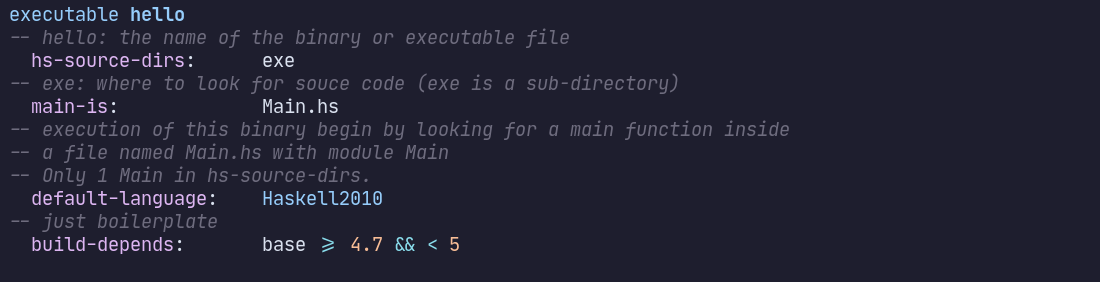
\includegraphics[width = 16cm]{images/stanza}

  Executables are applications that the operating system will run directly, while software
  libraries are code arranged in a manner so that they can be reused by the compiler in the
  building of other libraries and programs.
  {\fontfamily{ptm}\selectfont a }




\end{document}
